\subsubsection{Rouson's patterns}\label{sec:rouson}
The book by Rouson, Xia and Xu~\cite{rousonxiaxu} could be seen as template for designing and writing the
software to be written for \nep, since it starts with an introduction to object-oriented programming
and finishes with a description of the Morfeus multiphysics framework aimed ultimately at Exascale HPC.
Since most code examples are presented in both languages, the book may also be regarded as a `Rosetta stone'
for scientific programming in C++ and Fortran~2003, see \Tab{oopnomen}, and including
a chapter~(\S\,11) devoted to discussion of the interoperability of the two languages.
Notably too, Rouson~et~al~\cite[\S,4.2.3]{rousonxiaxu} describe how one of the first examples of object-oriented
scientific programming, described in the book by by Gardner and Manduchi~\cite{gardnermanduchi},
is an application in nuclear fusion, namely a data acquisition code written in Java.

\begin{table}[h]
\begin{center}
\caption{Rouson, Xia and Xu as a `Rosetta Stone' -- Table~2.1 from~\cite{rousonxiaxu} 
on Object-Oriented Programming nomenclature.\label{tab:oopnomen}}
\begin{tabular}{|p{5cm}|p{5cm}|p{5cm}|}
\hline
Fortran 2003 & C++ & General \\
\hline
Derived type & Class & Abstract data type~(ADT) \\
Component & Data member & Attribute \\
Class & Dynamic Polymorphism & \\
select type & (emulated via dynamic\_cast) &\\
Type-bound procedure & Virtual Member function & Method, operation \\
Parent type & Base class & Parent class \\
Extended type & Subclass & Child class \\
Module & Namespace & Package \\
Generic interface & Function overloading & Static polymorphism \\
Final procedure & Destructor &\\
Defined operator & Overloaded operator & \\
Defined assignment & Overloaded assignment operator & \\
Deferred procedure binding & Pure virtual member function & Abstract method \\
Procedure interface & Function prototype & Procedure signature \\
Intrinsic type/procedure & Primitive type/procedure & Built-in type/procedure \\
\hline
\end{tabular}
\end{center}
\end{table}

In this report, the focus is on design patterns,
to which concept Rouson~et~al~\cite{rousonxiaxu} contribute the idea of  ``domain-specific design patterns",
where the domain is the scientific one encompassing \nep. Rouson and coworkers also describe language-specific
design patterns, namely {\it Surrogate}~\cite[\S\,7]{rousonxiaxu} for Fortran~2003 and
{\it Compute Globally, Return Locally}~(CGRL)~\cite{Ha15High} for
Co-array Fortran~(CAF). These are necessary because of deficiencies in the programming language(s)
and will not be further discussed.

In Rouson~et~al~\cite[\S\,5]{rousonxiaxu}, the concept of object (which they pedantically
describe as a language-specific pattern because it is not fundamental to either the Fortran~2003 or C++ languages)
underlies their discussion of design patterns. The book also emphasises the importance of UML
in describing patterns~\cite[\S\,B]{rousonxiaxu}.
\Tab{rousonpats} which is reproduced from~\cite{rousonxiaxu}, summarises
the generic design patterns found useful for scientific work in the book, either directly or because
they inspired related scientific design patterns.

\begin{table}[h]
\begin{center}
\caption{Useful Go4 design patterns and summary descriptions -- 
Table~4.1 from~\cite{rousonxiaxu}, augmented with pointers
to sections in the book \label{tab:rousonpats}}
\begin{tabular}{|p{3cm}|p{12cm}|}
\hline
Pattern	& Allow Varying of  \\
\hline
{\it Factory Method} & Subclass of instantiated object~\S\,9  \\
{\it Proxy} & Location or method of accessing an object  \\
{\it Composite} & Object structure and composition~(\S\,9.2)  \\
{\it Facade} & Interface to a subsystem~\S\,6 \\
{\it Iterator} & How an aggregate's elements are accessed~\S\,5.4  \\
{\it Mediator} & How and which objects interact with each other~\S\,8  \\
{\it Strategy} & An algorithm~\S\,7  \\
{\it Template Method} & Step(s) of an algorithm~\S\,9.4  \\
{\it Singleton} & Global variable(s)~\S\,9.3  \\
{\it Abstract Factory} & Factory method~\S\,9  \\
\hline
\end{tabular}
\end{center}
\end{table}


The {\it Strategy} pattern is shown to be directly useful in scientific programming, with the example of
enabling an easy switch between different methods for integrating a PDE forward in time, such as
forward Euler or $2^{nd}$~order Runge-Kutta. The next novelty arises from the perceived need for a
multiphysics program with `separation of concerns' to be adaptable at the level of mathematical abstraction
of the vector calculus, or more precisely the tensor calculus. This leads to the introduction
in ref~\cite[\S\,6]{rousonxiaxu}
of the Abstract~Data~Type or ADT~calculus for PDEs, referred to as `abstract calculus' where say
partial derivative with respect
to time~$(\partial/\partial t)$ and Laplacian operator~$\nabla^2$ have special representations in software,
cf.\ overloading operators. Externally, the {\it Abstract Calculus} pattern exhibits many aspects of the {\it Facade}
design pattern, whereas internally the separate operators may be regarded as {\it Template Methods}.

There is criticism of the {\it Mediator} pattern see~\Fig{mediator}, because
of the linear growth in its complexity with the number of objects it has to connect, hence
the introduction of the {\it Puppeteer} pattern, see \Fig{puppet}. The key distinction is that the connected
objects need know nothing about the {\it Puppeteer}.
\begin{figure}
\centerline{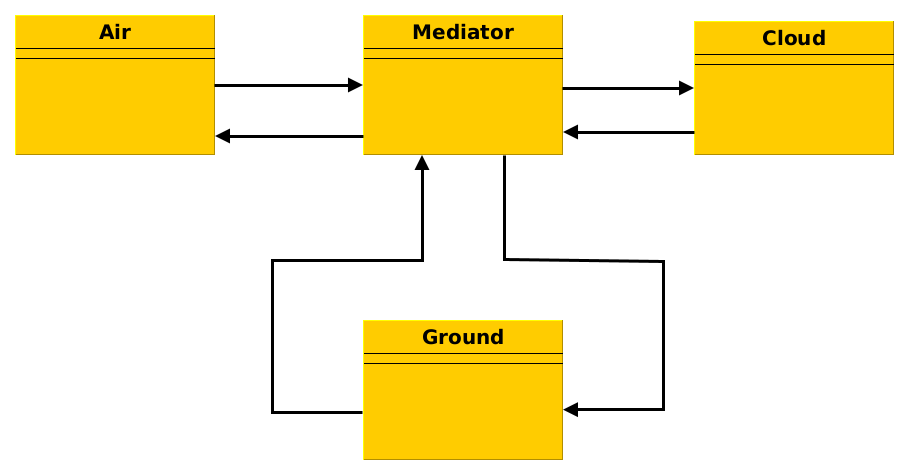
\includegraphics[width=12cm]{../png/mediator2_wa}}
\caption{UML class diagram for the {\it Mediator} pattern showing application to the problem of
accessing an atmospheric state defined by separate data describing air, cloud and ground properties -- After
Fig.~8.1 from \protect{\cite{rousonxiaxu}}.\label{fig:mediator}}
\end{figure}
\begin{figure}
(a)\centerline{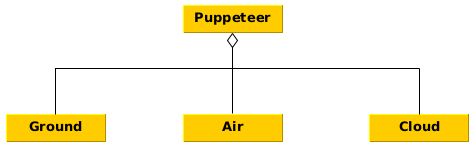
\includegraphics[width=10cm]{../png/puppeteer_wa}}
\\(b)\centerline{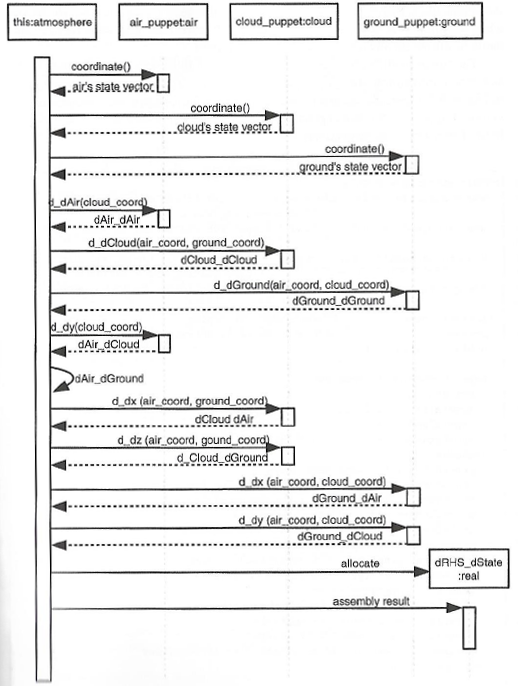
\includegraphics[width=10cm]{../png/puppetseq}}
\caption{At top~(a), UML class diagram for the {\it Puppeteer} pattern -- after Fig.~8.2 from \protect{\cite{rousonxiaxu}}.
Below~(b), UML sequence diagram for the {\it Puppeteer} pattern -- Fig.~8.3 from \protect{\cite{rousonxiaxu}},
when specifically derivative information is required so the puppeteer can form a Jacobian matrix.\label{fig:puppet}}
\end{figure}


The application of {\it Abstract Factory} pattern to {\it Abstract Calculus} is to define
discrete properties to be applied to a field in order to solve a PDE. Rouson~et~al give the example of
the flow~$u(x,t)$ as a solution to Burgers' equation, as the `Field' returned by reference from
the {\it Factory Method} create() in~\Fig{factory},
where the {\it Abstract Factory} {\it \bf FieldFactory} uses the concrete Periodic6thFactory which
aggregates (discrete) periodic boundary conditions with a $6^{th}$-order Pad\'{e} approximation.
The point is that other boundary conditions and approximations may be easily substituted for
periodic and $6^{th}$-order Pad\'{e} respectively, but the
create() interface remains the same. Indeed strictly speaking, these other substitutions  must be available
to satisfy the definition that an {\it Abstract Factory} is capable of creating a family of related objects.

\begin{figure}
\centerline{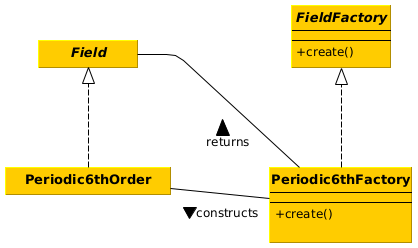
\includegraphics[width=12cm]{../png/factory_wa}}
\caption{UML class diagram for the {\it Abstract Factory} pattern showing application to solving a PDE -- after Fig.~9.1 from \protect{\cite{rousonxiaxu}}.\label{fig:factory}}
\end{figure}


Software described in the Rouson~et~al book apparently culminates with the Morfeus framework for 
multiphysics. The reason this otherwise seemingly very relevant framework is not described in the report~\cite{y2re312}
is that on close inspection, what ref~\cite{rousonxiaxu} contains is more a proposal to implement the design
patterns in the book than a finished project. The only related public repository found was actually set up very recently~(2020)
by Rouson, and contains Fortran~2003 code only~\cite{morfeuswebsite}.
%Probably this incorporates the Sandia code  presumably developed throughout the 2010s, mentioned at
%https://crf.sandia.gov/combustion-research-facility/reacting-flow/math/codes/

%shared\_ptr cf. Soustrop's tour
%S12.3 Morfeus framework - calls user code
%
%Coordinate-free programming (CFP)
